\section{Modelos que expressam a relação IDF}

As relações intensidade-duração-frequência podem ser expressas matematicamente, ou seja, equações propostas que representam a quantidade máxima de uma chuva. A definição do modelo que representa as chuvas intensas, utilizado em cada trabalho, deve ser de fácil manuseio, mantendo a segurança em seus resultados que devem ser o mais próximo à realidade \cite{interpolacao-chuva}. A Figura \ref{fig:curva-idf} exemplifica as curvas características de uma equação IDF.

\begin{figure}[h]
    \caption{Representação das curvas características de uma equação IDF}
    \centering
    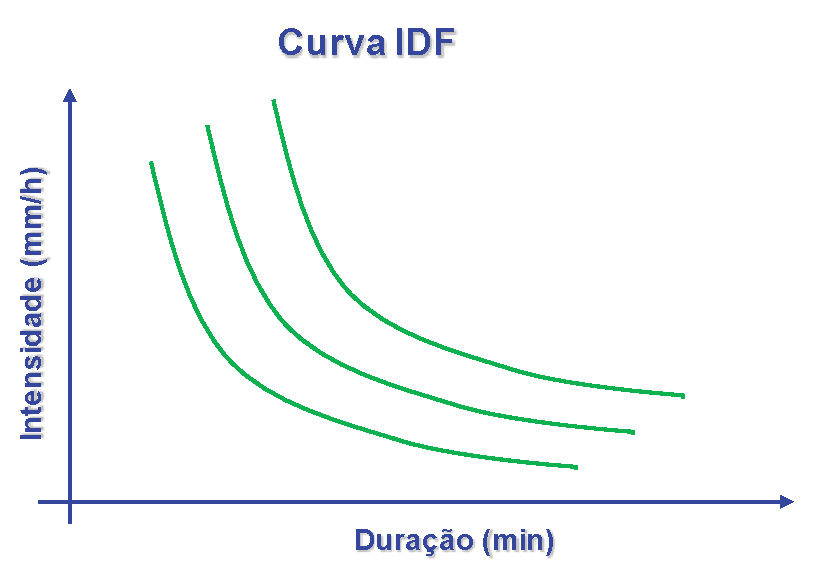
\includegraphics[width=0.7\textwidth]{Textuais/Figuras/curva-idf.pdf}
    \fonte{Autores}
    \label{fig:curva-idf}
\end{figure}

Segundo \citeonline{hidrologia-aplicada}, o modelo matemático clássico mais utilizado no Brasil é expresso pela Equação \ref{eq:equacao-geral}.

Em situações onde a escassez de dados é muito grande, evidenciam a importância da comparação entre vários modelos que representam a relação IDF, podendo resultar em informações confiáveis e precisas. Em seu trabalho, os autores \citeonline{interpolacao-chuva} utilizam modelo exponencial, representado pela Equação \ref{eq:modelo-linear}, e linear, representado pela Equação \ref{eq:exponencial}.

\begin{equation}
\label{eq:modelo-linear}
    i = e^{B + D \times T_r^x + E (Ln(t))^2 + \epsilon}
\end{equation}

Em que:

i = Intensidade de chuva [mm/h]

$B$, $D$, $x$, $E$ = Parâmetros de ajuste estatístico, referentes a cada localidade

$\epsilon$ = Erro produzido pelo ajuste

t = Duração [min]


\begin{equation}
\label{eq:exponencial}
    i = A_1 \times Ln(T_r) + B_1 \times Ln(t) + C_1[Ln(t)]^2 + D_1Ln(T_r)Ln(t) + \epsilon
\end{equation}

Em que:

$A_1$, $B_1$, $C_1$, $D_1$ = Parâmetros de ajuste estatístico, referentes a cada localidade \\

\par \citeonline{interpolacao-chuva} concluíram que o modelo exponencial produziu erros menores, gerando melhores aproximações da intensidade máxima de chuvas. O modelo linear, apesar de possuir um coeficiente de determinação $R^2$ superior a 0,99, não foi considerado confiável para utilização em estudos de chuvas intensas, pois apresenta os maiores erros médios e, também, a maior amplitude de erros comparado ao modelo exponencial.

\citeonline{chuvas-brasil}, em seu trabalho de determinação das curvas IDF, realizou o ajuste do modelo representado pela Equação \ref{eq:pfafstetter}.

\begin{equation}
\label{eq:pfafstetter}
    P=R[\alpha \times t + b \times Log(1 + c \times t)]
\end{equation}

Em que:

P = Precipitação pluvial máxima (mm)

$\alpha$, b, c = Parâmetros de ajuste local

R = Fator de probabilidade \\

\par O fator R é definido pela Equação \ref{eq:fator-r}.

\begin{equation}
\label{eq:fator-r}
    R = T_r^{(\alpha + \frac{\beta}{T_r})^{0.25}}
\end{equation}

Em que:

$\alpha$ e $\beta$ = Parâmetros que dependem da duração da precipitação \\

\par A Equação \ref{eq:pfafstetter} fornece a precipitação para período de retorno de 1 ano e a Equação \ref{eq:fator-r} permite estimar a chuva para outros tempos de retorno \cite{tucci1993}.

\citeonline{bt} detalharam a metodologia de Bell, que relaciona a precipitação máxima para um tempo de duração definido e período de retorno a uma precipitação padrão de 60 minutos de duração e 2 anos de período de retorno, a Equação \ref{eq:met-bell} representa o resultado obtido pelos autores.

\begin{equation}
\label{eq:met-bell}
    h_{(t,T_r)} = (\alpha \times Ln(T_r) + a_1)(a_2 \times t_d^b - a_3)h_{(60,2)}
\end{equation}

Em que:

$h_{(t, T_r)}$ = Altura de chuva com duração $t_d$ e período de retorno $T_r$ [mm]

$\alpha$, $a_1$, $a_2$, $a_3$, b = Parâmetros de ajuste do modelo

$h_{(60,2)}$ = Precipitação intensa com duração 60 minutos e período de retorno de 2 anos \\

\par De acordo com \citeonline{sampaio}, a metodologia Bell se baseia em séries de chuva, observadas em todo globo terrestre, destacando que o valor máximo das chuvas está relacionando a regiões convectivas com características parecidas no mundo todo; assinalando isso com uma desvantagem do método, uma vez que as equações são geradas de valores médios e não específicos para uma determinada região. O autor, também, apontou como desvantagem que o valor da precipitação máxima obtida é válido apenas para durações entre 5 a 120 minutos.

\citeonline{interpolacao-chuva} comentaram que a principal característica do método de Bell é o ajuste da equação, que pode ser regionalizada e que alguns autores optam pelo emprego do modelo de Bell, para o Brasil, atribuindo valores fixos aos parâmetros de ajuste, variando apenas o período de retorno e a intensidade da chuva. %comentar sobre quais são empiricos e quais são teóricos
    
\citeonline{interpolacao-chuva} realizaram ajustes do modelo de Bell para as seguintes regiões: Norte, Sul, Centro, Leste e Triângulo Mineiro e alcançaram um desvio inferior a 8\% entre os valores empíricos e teóricos.

O método de Bell mostra-se adequado para estimar as máximas precipitações de curta duração, sendo uma opção na determinação das chuvas críticas de projeto quando as séries disponíveis contém poucos anos de observação \cite{goias}. \citeonline{mt} aplicaram o modelo de Bell para plataforma de coleta de dados (PCD) no Estado do Mato Grosso e verificaram que, comparado com as relações IDF elaboradas pelo modelo clássico (apresentado na Equação \ref{eq:equacao-geral}), o modelo de Bell superestimou a chuva de projeto.

\citeonline{rainfall} sugeriu uma equação IDF utilizando três alturas de precipitação: chuva com duração de 1 hora e período de retorno de 10 anos; chuva com duração de 24 horas e período de retorno de 10 anos; chuva com duração de 1 hora e período de retorno de 100 anos. De acordo com o autor, verificou-se que, nas precipitações a partir da duração de 2 horas, as relações de duração em relação à chuva de 24 horas variaram em função da relação da chuva de 1 hora e à de 24 horas. A Equação \ref{eq:chen}, proposta por \citeonline{rainfall}, foi desenvolvida para as séries anuais.

\begin{equation}
\label{eq:chen}
    h_{(td,T_r)} = \frac{a \times h_{(1,10)} Log(10^{2-w}Ln(\frac{T_r}{T_r-1})^{1-w})}{(d+b)^c} \frac{d}{60}
\end{equation}

Em que:

$h_{(td, T_r)}$ = Altura de chuva com duração d em minutos [mm]

$h_{(1,10)}$ = Altura de chuva com uma hora de duração e período de retorno de 10 anos [mm]

a, b, c = Parâmetros obtidos em função da relação $h_{(1, T_r)}$

w = Relação entre a chuva de uma hora de duração e período de retorno de 100 anos.

